\documentclass[tikz,border=4pt]{standalone}
\usepackage{amsmath}
\usetikzlibrary{decorations.pathreplacing}
\renewcommand{\familydefault}{\sfdefault}

\begin{document}
	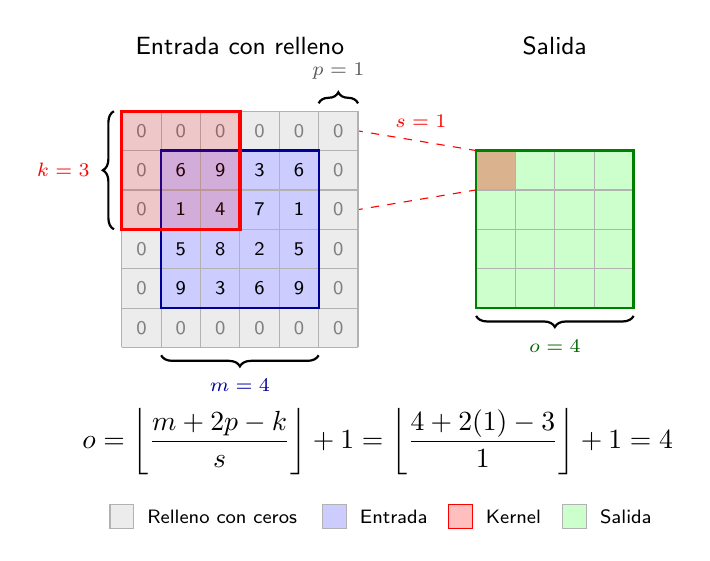
\begin{tikzpicture}[scale=0.5, every node/.style={font=\scriptsize},
		brace/.style={decorate, decoration={brace, amplitude=4pt}, thick}]
		
		% Kernel-to-output mapping (drawn first so the grids cover it)
		\draw[dashed, red] (3,6) -- (9,5);
		\draw[dashed, red] (3,3) -- (9,4);
		\node[red] at (7.6,5.75) {$s=1$};
		
		% ---------- Padded input (m = 4, p = 1 -> 6x6) ----------
		% Celdas de relleno con ceros
		\foreach \x in {0,...,5}
		\foreach \y in {0,...,5} {
			\fill[gray!15] (\x,\y) rectangle ++(1,1);
			\node[gray] at (\x+0.5,\y+0.5) {0};
		}
		% Celdas de la entrada original
		\foreach \x in {1,...,4}
		\foreach \y in {1,...,4} {
			\pgfmathtruncatemacro{\v}{mod(3*\x+5*\y,9)+1}
			\fill[blue!20] (\x,\y) rectangle ++(1,1);
			\node at (\x+0.5,\y+0.5) {\v};
		}
		\draw[step=1, gray!60] (0,0) grid (6,6);
		\draw[thick, blue!60!black] (1,1) rectangle (5,5);
		
		% Kernel (k = 3) at top-left position
		\fill[red, opacity=0.15] (0,3) rectangle (3,6);
		\draw[very thick, red] (0,3) rectangle (3,6);
		
		% Braces
		\draw[brace] (-0.2,3) -- (-0.2,6) node[midway, left=5pt, red] {$k=3$};
		\draw[brace] (5,6.2) -- (6,6.2) node[midway, above=5pt, gray!70!black] {$p=1$};
		\draw[brace] (5,-0.2) -- (1,-0.2) node[midway, below=5pt, blue!60!black] {$m=4$};
		
		\node[above] at (3,7.2) {\small Entrada con relleno};
		
		% ---------- Output (o = 4) ----------
		\foreach \x in {0,...,3}
		\foreach \y in {0,...,3}
		\fill[green!20] (9+\x,1+\y) rectangle ++(1,1);
		\fill[red, opacity=0.3] (9,4) rectangle (10,5);
		\draw[step=1, gray!60, shift={(9,1)}] (0,0) grid (4,4);
		\draw[thick, green!50!black] (9,1) rectangle (13,5);
		
		\draw[brace] (13,0.8) -- (9,0.8) node[midway, below=5pt, green!40!black] {$o=4$};
		\node[above] at (11,7.2) {\small Salida};
		
		
		% ---------- Arithmetic ----------
		\node at (6.5,-2.4) {\normalsize
			$o = \left\lfloor \dfrac{m + 2p - k}{s} \right\rfloor + 1
			= \left\lfloor \dfrac{4 + 2(1) - 3}{1} \right\rfloor + 1 = 4$};
		
		% ---------- Legend ----------
		\begin{scope}[shift={(-0.3,-4.6)}]
			\fill[gray!15] (0,0) rectangle (0.6,0.6); \draw[gray!60] (0,0) rectangle (0.6,0.6);
			\node[right] at (0.7,0.3) {Relleno con ceros};
			\fill[blue!20] (5.4,0) rectangle (6.0,0.6); \draw[gray!60] (5.4,0) rectangle (6.0,0.6);
			\node[right] at (6.1,0.3) {Entrada};
			\fill[red!25] (8.6,0) rectangle (9.2,0.6); \draw[red] (8.6,0) rectangle (9.2,0.6);
			\node[right] at (9.3,0.3) {Kernel};
			\fill[green!20] (11.5,0) rectangle (12.1,0.6); \draw[gray!60] (11.5,0) rectangle (12.1,0.6);
			\node[right] at (12.2,0.3) {Salida};
		\end{scope}
	\end{tikzpicture}
\end{document}